\documentclass{beamer}
\usepackage[utf8]{inputenc}

\usetheme{Madrid}
\usecolortheme{default}
\usepackage{amsmath,amssymb,amsfonts,amsthm}
\usepackage{txfonts}
\usepackage{tkz-euclide}
\usepackage{listings}
\usepackage{adjustbox}
\usepackage{array}
\usepackage{tabularx}
\usepackage{gvv}
\usepackage{lmodern}
\usepackage{circuitikz}
\usepackage{tikz}
\usepackage{graphicx}

\setbeamertemplate{page number in head/foot}[totalframenumber]

\usepackage{tcolorbox}
\tcbuselibrary{minted,breakable,xparse,skins}



\definecolor{bg}{gray}{0.95}
\DeclareTCBListing{mintedbox}{O{}m!O{}}{%
  breakable=true,
  listing engine=minted,
  listing only,
  minted language=#2,
  minted style=default,
  minted options={%
    linenos,
    gobble=0,
    breaklines=true,
    breakafter=,,
    fontsize=\small,
    numbersep=8pt,
    #1},
  boxsep=0pt,
  left skip=0pt,
  right skip=0pt,
  left=25pt,
  right=0pt,
  top=3pt,
  bottom=3pt,
  arc=5pt,
  leftrule=0pt,
  rightrule=0pt,
  bottomrule=2pt,

  colback=bg,
  colframe=orange!70,
  enhanced,
  overlay={%
    \begin{tcbclipinterior}
    \fill[orange!20!white] (frame.south west) rectangle ([xshift=20pt]frame.north west);
    \end{tcbclipinterior}},
  #3,
}
\lstset{
    language=C,
    basicstyle=\ttfamily\small,
    keywordstyle=\color{blue},
    stringstyle=\color{orange},
    commentstyle=\color{green!60!black},
    numbers=left,
    numberstyle=\tiny\color{gray},
    breaklines=true,
    showstringspaces=false,
}
%------------------------------------------------------------
%This block of code defines the information to appear in the
%Title page
\title %optional
{3.3.15}
\date{\today}
%\subtitle{A short story}

\author % (optional)
{Shivam Sawarkar \\ AI25BTECH11031}



\begin{document}


\frame{\titlepage}
\begin{frame}{Question}
    Construct a triangle ABC in which $BC = 7 cm$, and median $AD = 5 cm$, $\angle A=60^\circ$. Write the steps of construction also.
\end{frame}

\begin{frame}{Solution}
    \begin{align}
\vec{B}=\myvec{0\\0},\qquad 
\vec{C}=\myvec{7\\0},\qquad 
\vec{D}=\myvec{3.5\\0}.
\end{align}

Since $AD=5$, point $\vec{A}$ lies on the circle with center $\vec{D}$ and radius 5.  
We parametrize:
\begin{align}
\vec{A}=\vec{D}+5\myvec{\cos\theta\\ \sin\theta}
=\myvec{3.5+5\cos\theta\\[4pt]5\sin\theta}.
\end{align}

Define the vectors
\begin{align}
\vec{c}=\vec{AB}=\vec{B}-\vec{A}
=\myvec{-3.5-5\cos\theta\\ -5\sin\theta},\\ 
\vec{b}=\vec{AC}=\vec{C}-\vec{A}
=\myvec{3.5-5\cos\theta\\ -5\sin\theta}.
\end{align}
\end{frame}

\begin{frame}{Solution}
    \textbf{Angle condition:}  
\begin{align}
\vec{c}^\top \vec{b}=\norm{c}\norm{b}\cos60^\circ
=\dfrac{1}{2}\norm{c}\norm{b}
\end{align}

Compute the dot product:
\begin{align}
\vec{c}^\top \vec{b}
=(-3.5-5\cos\theta)(3.5-5\cos\theta)+(-5\sin\theta)(-5\sin\theta)
=\frac{51}{4}.
\end{align}

Hence
\begin{align}
\norm{b}\norm{c}=\frac{51}{2}.
\end{align}

Now,
\begin{align}
\norm{c}^2=\dfrac{149}{4}+35\cos\theta,\qquad
\norm{b}^2=\dfrac{149}{4}-35\cos\theta.
\end{align}

Therefore,
\begin{align}
(\norm{c}\norm{b})^2
=\brak{\dfrac{149}{4}}^2-(35\cos\theta)^2.
\end{align}
\end{frame}

\begin{frame}{Solution}
    Substituting $\norm{c}\;\norm{b}=\dfrac{51}{2}$,
\begin{align}
\brak{\dfrac{51}{2}}^2=\brak{\dfrac{149}{4}}^2-(35\cos\theta)^2,
\end{align}
\begin{align}
\cos^2\theta=\frac{11797}{19600}.
\end{align}

Thus,
\begin{align}
\cos\theta=\pm\frac{\sqrt{11797}}{140},\qquad
\sin\theta=\pm\frac{\sqrt{7803}}{140}.
\end{align}

Finally, coordinates of $A$ are
\begin{align}
\vec{A}=\myvec{
\dfrac{7}{2}\pm\dfrac{\sqrt{11797}}{28}\\ 
\pm\dfrac{\sqrt{7803}}{28}
}.
\end{align}
\end{frame}

\begin{frame}{Plot}
    \begin{figure}
        \centering
        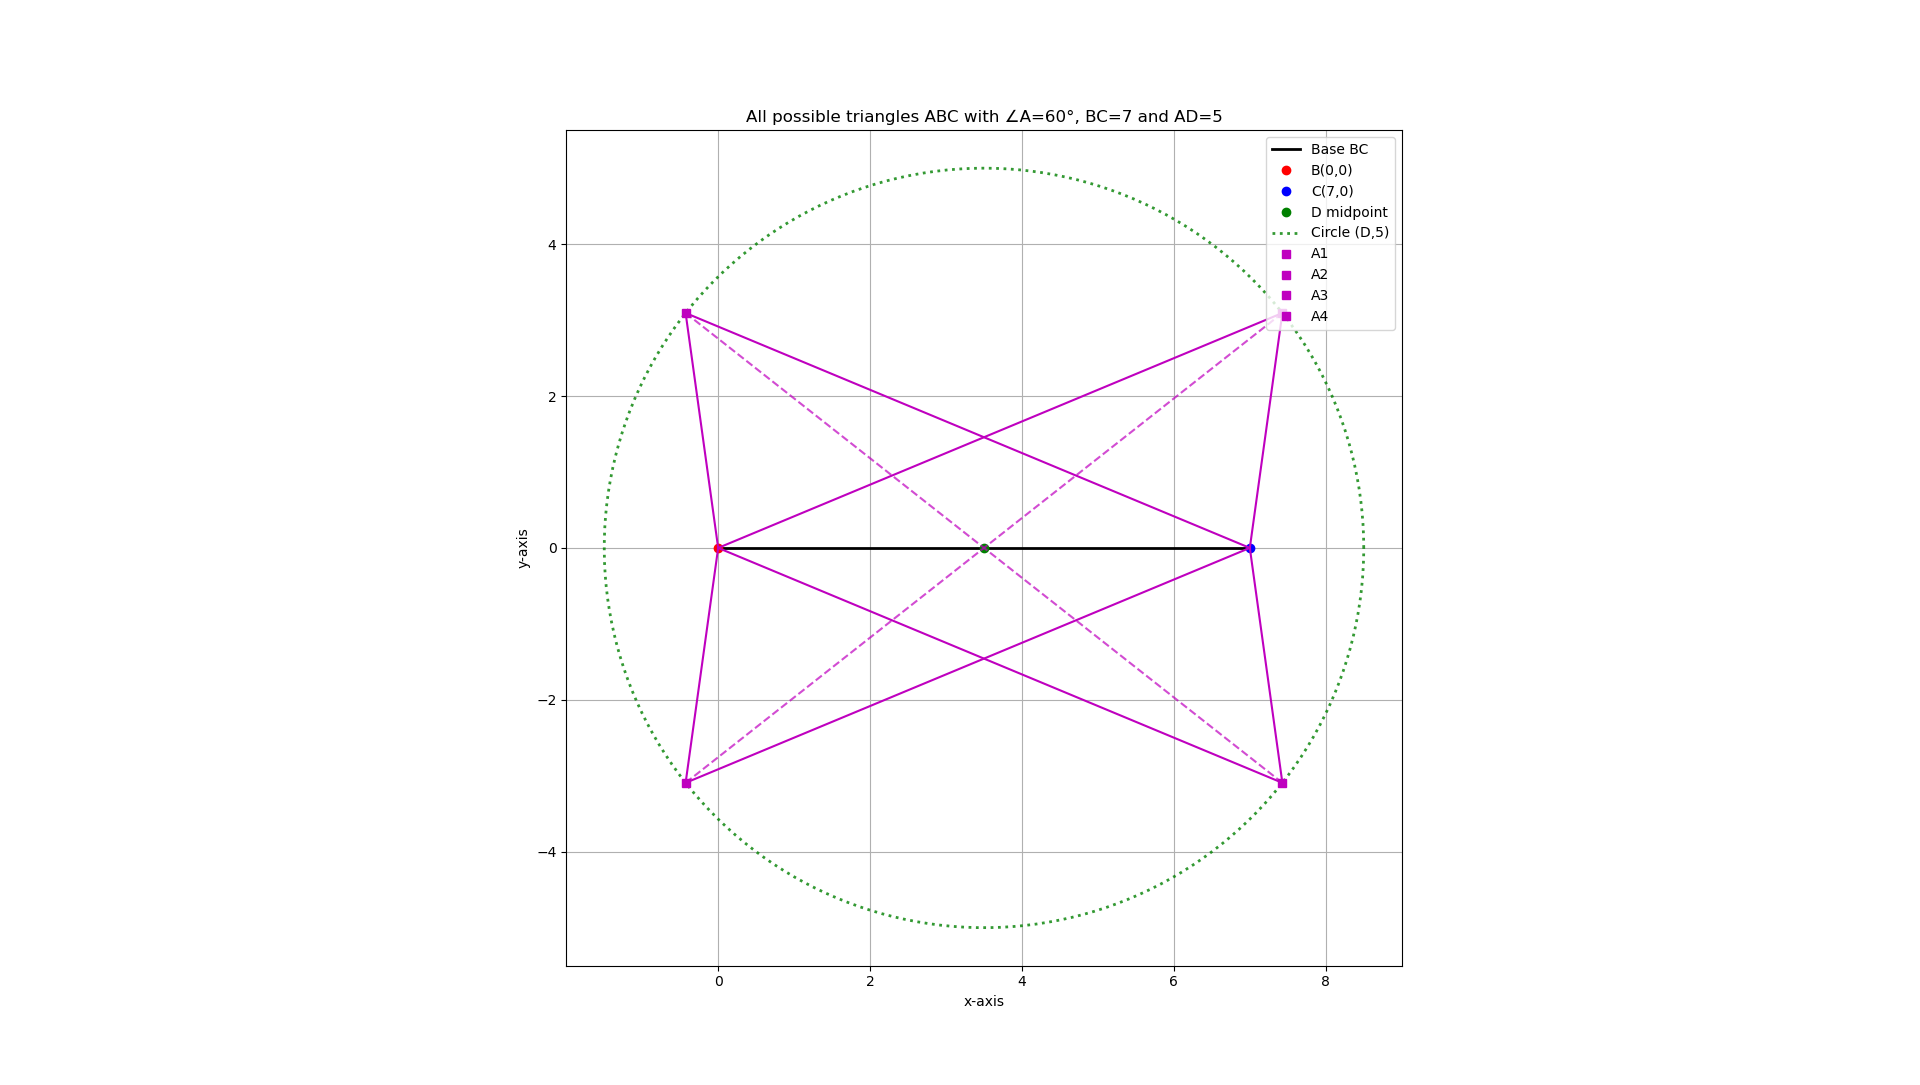
\includegraphics[width=1\linewidth]{figs/plot6.png}
        \caption{}
        \label{fig:placeholder}
    \end{figure}
\end{frame}

\begin{frame}[fragile]{C Code}
    \begin{verbatim}
#ifndef TRIANGLE_H
#define TRIANGLE_H

#include <math.h>
#include <stdio.h>

// Struct for a point
typedef struct {
    double x, y;
} Point;
// Function to compute intersections of two circles
__attribute__((visibility("default")))
int circle_intersections(Point c1, double r1, Point c2, double r2, Point *p1, Point *p2) {
    double dx = c2.x - c1.x;
    double dy = c2.y - c1.y;
    double d = hypot(dx, dy);
    \end{verbatim}
\end{frame}

\begin{frame}[fragile]{C Code}
    \begin{verbatim}
    if (d > r1 + r2 || d < fabs(r1 - r2) || d == 0) {
        return 0; // no intersection
    }

    double a = (r1*r1 - r2*r2 + d*d) / (2*d);
    double h = sqrt(fmax(r1*r1 - a*a, 0));
    double xm = c1.x + a*dx/d;
    double ym = c1.y + a*dy/d;
    double rx = -dy * (h/d);
    double ry = dx * (h/d);

    p1->x = xm + rx;
    p1->y = ym + ry;
    p2->x = xm - rx;
    p2->y = ym - ry;

    return 2; // two intersections
}

#endif
    \end{verbatim}
\end{frame}

\begin{frame}[fragile]{C Code}
    \begin{verbatim}
#include <stdio.h>
#include <math.h>
#include "solution.h"

int main() {
    double BC, AD, angleA;
    printf("Enter length BC: ");
    scanf("%lf", &BC);
    printf("Enter length of median AD: ");
    scanf("%lf", &AD);
    printf("Enter angle A (in degrees): ");
    scanf("%lf", &angleA);

    Point B = {0, 0};
    Point C = {BC, 0};
    Point D = {(B.x + C.x)/2, (B.y + C.y)/2};
    \end{verbatim}
\end{frame}

\begin{frame}[fragile]{C Code}
    \begin{verbatim}
// Circle with center D and radius AD
    double r1 = AD;

    // Angle condition: circumcircle with radius BC/(2*sinA)
    double A_rad = angleA * M_PI / 180.0;
    double R = BC / (2.0 * sin(A_rad));

    // Two possible centers of the angle-locus circle
    Point O1 = {D.x, D.y + R};
    Point O2 = {D.x, D.y - R};

    Point p1, p2;

    printf("\nPossible coordinates of A:\n");
    \end{verbatim}
\end{frame}

\begin{frame}[fragile]{C Code}
    \begin{verbatim}
    // Check intersections for O1
    if (circle_intersections(D, r1, O1, R, &p1, &p2)) {
        printf("A1 = (%.3f, %.3f)\n", p1.x, p1.y);
        printf("A2 = (%.3f, %.3f)\n", p2.x, p2.y);
    }

    // Check intersections for O2
    if (circle_intersections(D, r1, O2, R, &p1, &p2)) {
        printf("A3 = (%.3f, %.3f)\n", p1.x, p1.y);
        printf("A4 = (%.3f, %.3f)\n", p2.x, p2.y);
    }

    return 0;
}
    \end{verbatim}
\end{frame}

\begin{frame}[fragile]{Python Code}
    \begin{verbatim}
import math

class Point:
    def __init__(self, x, y):
        self.x = x
        self.y = y

def circle_intersections(c1, r1, c2, r2):
    dx = c2.x - c1.x
    dy = c2.y - c1.y
    d = math.hypot(dx, dy)

    if d > r1 + r2 or d < abs(r1 - r2) or d == 0:
        return []  # no intersection
    \end{verbatim}
\end{frame}

\begin{frame}[fragile]{Python Code}
    \begin{verbatim}
    a = (r1*r1 - r2*r2 + d*d) / (2*d)
    h = math.sqrt(max(r1*r1 - a*a, 0))
    xm = c1.x + a*dx/d
    ym = c1.y + a*dy/d
    rx = -dy * (h/d)
    ry = dx * (h/d)

    p1 = Point(xm + rx, ym + ry)
    p2 = Point(xm - rx, ym - ry)

    return [p1, p2]

# Input
BC = float(input("Enter length BC: "))
AD = float(input("Enter length of median AD: "))
angleA = float(input("Enter angle A (in degrees): "))
    \end{verbatim}
\end{frame}

\begin{frame}[fragile]{Python Code}
    \begin{verbatim}
# Points B, C, D
B = Point(0, 0)
C = Point(BC, 0)
D = Point((B.x + C.x) / 2, (B.y + C.y) / 2)

# Circle 1: center D, radius AD
r1 = AD

# Angle condition: circumcircle with radius BC/(2*sinA)
A_rad = math.radians(angleA)
R = BC / (2.0 * math.sin(A_rad))

# Two possible centers of angle-locus circle
O1 = Point(D.x, D.y + R)
O2 = Point(D.x, D.y - R)
    \end{verbatim}
\end{frame}

\begin{frame}[fragile]{Python Code}
    \begin{verbatim}
print("\nPossible coordinates of A:")

# Intersections with O1 circle
sol1 = circle_intersections(D, r1, O1, R)
for i, p in enumerate(sol1, start=1):
    print(f"A{i} = ({p.x:.3f}, {p.y:.3f})")

# Intersections with O2 circle
sol2 = circle_intersections(D, r1, O2, R)
for i, p in enumerate(sol2, start=len(sol1)+1):
    print(f"A{i} = ({p.x:.3f}, {p.y:.3f})")

if __name__ == "__main__":
    main()
    \end{verbatim}
\end{frame}

\begin{frame}[fragile]{Python + C Code}
    \begin{verbatim}
import ctypes
import math

# Load the shared library
lib = ctypes.CDLL("./solution.so")

# Define Point struct for Python
class Point(ctypes.Structure):
    _fields_ = [("x", ctypes.c_double),
                ("y", ctypes.c_double)]

# Set argument and return types
lib.circle_intersections.argtypes = [Point, ctypes.c_double, Point, ctypes.c_double,
                                     ctypes.POINTER(Point), ctypes.POINTER(Point)]
lib.circle_intersections.restype = ctypes.c_int
    \end{verbatim}
\end{frame}

\begin{frame}[fragile]{Python + C Code}
    \begin{verbatim}
def circle_intersections(c1, r1, c2, r2):
    p1, p2 = Point(), Point()
    count = lib.circle_intersections(c1, r1, c2, r2,
                                     ctypes.byref(p1), ctypes.byref(p2))
    if count == 2:
        return [p1, p2]
    return []

def main():
    BC = float(input("Enter length BC: "))
    AD = float(input("Enter length of median AD: "))
    angleA = float(input("Enter angle A (in degrees): "))

    B = Point(0, 0)
    C = Point(BC, 0)
    D = Point((B.x + C.x) / 2, (B.y + C.y) / 2)
    \end{verbatim}
\end{frame}

\begin{frame}[fragile]{Python + C Code}
    \begin{verbatim}
    r1 = AD
    A_rad = math.radians(angleA)
    R = BC / (2.0 * math.sin(A_rad))

    O1 = Point(D.x, D.y + R)
    O2 = Point(D.x, D.y - R)

    print("\nPossible coordinates of A:")

    sol1 = circle_intersections(D, r1, O1, R)
    for i, p in enumerate(sol1, start=1):
        print(f"A{i} = ({p.x:.3f}, {p.y:.3f})")
    \end{verbatim}
\end{frame}

\begin{frame}[fragile]{Python + C Code}
    \begin{verbatim}
    sol2 = circle_intersections(D, r1, O2, R)
    for i, p in enumerate(sol2, start=len(sol1)+1):
        print(f"A{i} = ({p.x:.3f}, {p.y:.3f})")

if __name__ == "__main__":
    main()
    \end{verbatim}
\end{frame}





\end{document}